\documentclass[12pt]{article}
\usepackage[margin=0.2in]{geometry}
\usepackage{amssymb}
\usepackage{amsmath}
\usepackage{url}
\usepackage{bm}
\usepackage{color}
\usepackage{graphicx}
\usepackage{cite}
\usepackage{caption}
\usepackage{subcaption}
\usepackage{hyperref}
\usepackage[section]{placeins} %keeps floats in their own section

\hypersetup{
    colorlinks,
    citecolor=blue,
    filecolor=blue,
    linkcolor=blue,
    urlcolor=blue
}

%\title{Plots for Alpha Formation in Mostly Neutron Matter}
%\author{Cody L. Petrie}

\begin{document}
%\maketitle
%\tableofcontents
%\newpage

Here are the latest calculations for the alpha formation in mostly neutron matter. I've done some calculations at different densities, not all of which are finished, but this is what I have in Figure~\ref{fig:alpha}.
\begin{figure}[h!]
   \centering
   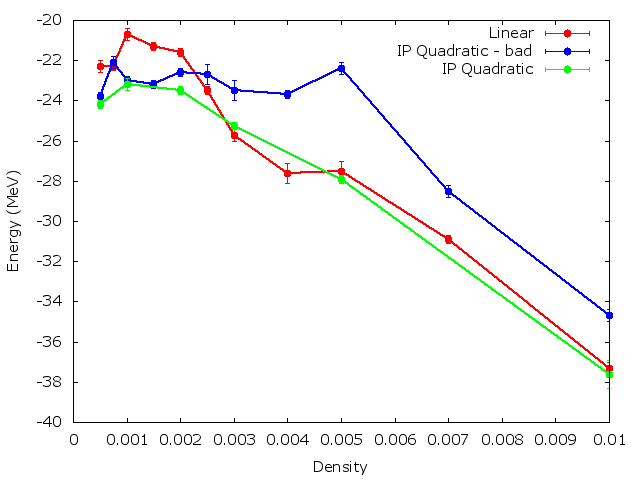
\includegraphics[width=0.60\textwidth]{../../alpha.png}
   \caption{Alpha energy calculated as $16\epsilon_{14n2p}-12\epsilon_{14n}$ where $\epsilon=E/A$.}
   \label{fig:alpha}
\end{figure}
It looks like the two correlations give about the same answer above $\rho=0.002$ fm$^{-3}$, and the quadratic (IP) correlations give more binding below that density.

I also did calculations at the same densities with just 2 neutrons and 2 protons for comparison and as you can see in figure~\ref{fig:alpha_and_2n2p} however the two correlations give about the same answer, so the extra neutrons must be sensative to the extra correlations of the quadratic. Figure~\ref{fig:alpha_and_2n2p} also compares the 2n2p calculations to the cluster calculations in Figure~\ref{fig:alpha}.
\begin{figure}[h!]
   \centering
   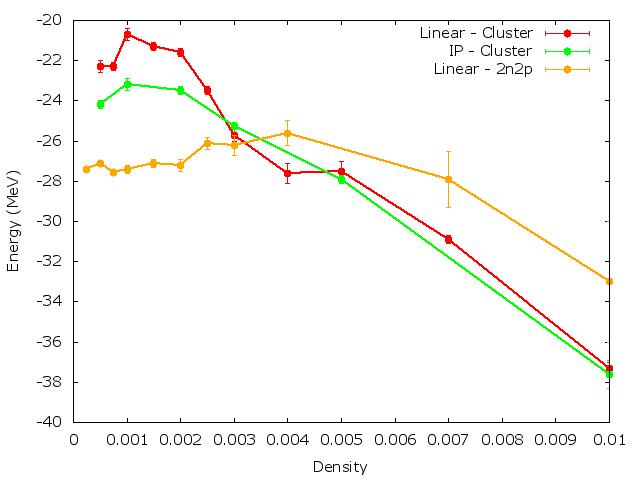
\includegraphics[width=0.60\textwidth]{../../alpha_and_2n2p.png}
   \caption{Energy of alpha particle calculated as a cluster in mostly neutron matter and 2 neutrons and 2 protons with both linear and IP correlations.}
   \label{fig:alpha_and_2n2p}
\end{figure}

I also plotted the separate pieces of the AV6' potential to see which pieces of the quadratic correlations mattered the most. Figure~\ref{fig:av6_alpha_linVSip} shows that the two pieces that differ the most are the OPE pieces, sigma-tau (vst in the plot) and tensor-tau (vtent in the plot). So this is good.
\begin{figure}[h!]
   \centering
   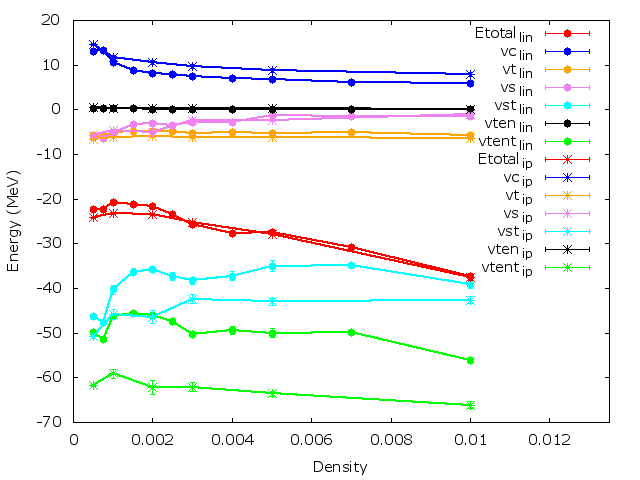
\includegraphics[width=0.60\textwidth]{../../av6_alpha_linVSip.png}
   \caption{Energy of alpha particle calculated as a cluster in mostly neutron matter and 2 neutrons and 2 protons with both linear and IP correlations.}
   \label{fig:av6_alpha_linVSip}
\end{figure}

I also compared the proton-proton correlations functions in Figure~\ref{fig:gpp_linVSip} and found that for the protons are more likely to be closer together for the quadratic correlations than for the linear correlations, adding proof that the quadratic correlations are important for the cluster formation. This is not true for the 2n2p calculations. As can be seen in Figure~\ref{fig:gpp_linVSip_alpha}
\begin{figure}[h!]
   \centering
   \begin{subfigure}{0.49\textwidth}
      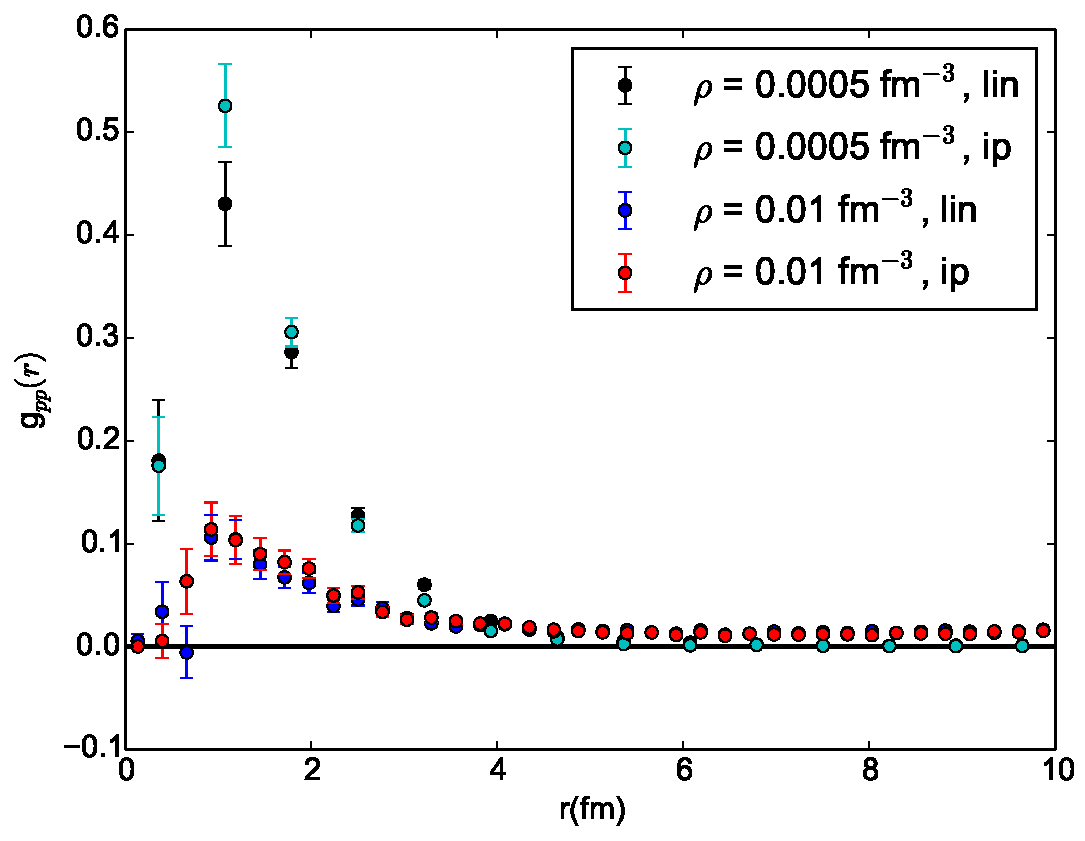
\includegraphics[width=\textwidth]{../../gpp_linVSip.pdf}
      \caption{$g_{pp}$ distribution for cluster calculations comparing linear and IP correlations for low and high densities.}
      \label{fig:gpp_linVSip}
   \end{subfigure}
   \begin{subfigure}{0.49\textwidth}
      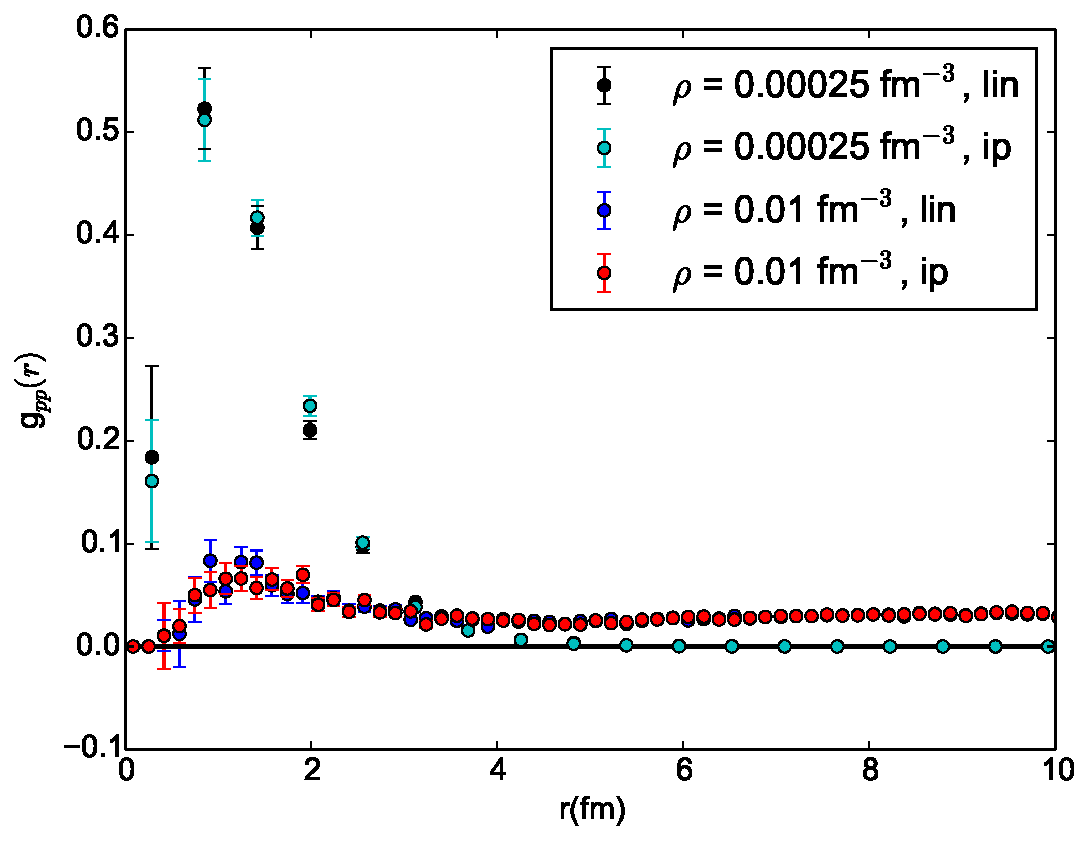
\includegraphics[width=\textwidth]{../../gpp_linVSip_alpha.pdf}
      \caption{$g_{pp}$ distribution for the 2n2p calculations comparing linear and IP correlations for low and high densities.}
      \label{fig:gpp_linVSip_alpha}
   \end{subfigure}
\end{figure}

\newpage
\section*{General Conclusions}
\begin{itemize}
   \item The quadratic correlations are important, but only when the alpha cluster is interacting with other particles, {\it i.e.} with the cluster calculations, but not the for 2n2p calculation.
   \item The piece of the potential that is effected most by the quadratic correlations are the OPE pieces.
   \item Both the ``flat" low density energies and the $g_{pp}$ calculations indicate that alpha clusters are forming at low densities.
\end{itemize}

\end{document}
